\documentclass{beamer}    % 14pt je nenujen
\usepackage[T1]{fontenc}
\usepackage[utf8]{inputenc}
\usepackage[slovene]{babel}
\usepackage{pgfpages}           % privat zapiski
\usepackage{amsfonts}
\usepackage{amsmath,amsthm}     % pravilen izpis v "math mode"
%\usepackage{hyperref}
\usepackage{graphicx}           % za slike
\usepackage{tikz}

%\hypersetup{hidelinks}

\setbeamertemplate{theorems}[ams style]             % numbered da brez bold 

\setbeameroption{hide notes}                        % samo prosojnice
%\setbeameroption{show only notes}                   % samo zapiski
%\setbeameroption{show notes on second screen=right}  % oboje

\usepackage{palatino}
\usefonttheme{serif}

%\usecolortheme{beetle} %ali beetle morda ali seagull 

\setbeamertemplate{navigation symbols}{} % izklop navigacije
\setbeamertemplate{footline}[frame number]{} % oštevilčenje
\setbeamertemplate{note page}{\pagecolor{yellow!5}\insertnote}

\newtheorem{izrek}{Izrek}
\newtheorem{trditev}[izrek]{Trditev}
\newtheorem{posledica}[izrek]{Posledica}
\newtheorem{definicija}[izrek]{Definicija}
\newtheorem{naloga}[izrek]{Naloga}
\newtheorem{resitev}[izrek]{Naloga}

\author{Tim Kalan}
\institute[FMF]{Fakulteta za matematiko in fiziko}
\title{
    Spodbujevano učenje pri igranju namiznih iger \\ 
    \large (angl. \textit{Reinforcement learning in board games})}
\date{\today} 



\begin{document}

\begin{frame}
    \titlepage
\end{frame}


\begin{frame}
    \frametitle{Strojno učenje}
    \begin{itemize}
        \item Nadzorovano učenje \textit{(npr. prepoznavanje števk)}
        \item Nenadzorovano učenje \textit{(npr. razvrščanje)}
        \item \textbf{Spodbujevano učenje}
    \end{itemize}
\end{frame}


\begin{frame}
    \frametitle{Motivacija: Instrumentalno pogojevanje}
    \begin{itemize}
        \item Tu bo slika 
        (http://www.edugyan.in/2017/03/edward-lee-thorndike-theory-of-learning.html, 
        https://en.wikipedia.org/wiki/Reinforcement)
        \item Lepa psihološko motivirana podlaga
        \item \textbf{Nagrade in kazni} 
    \end{itemize}

    \begin{figure}[b]
        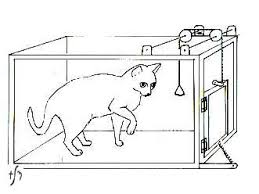
\includegraphics[scale=0.47]{slike/macka.jpg}
        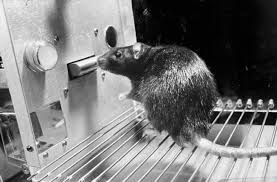
\includegraphics[scale=0.5]{slike/miska.jpg}
    \end{figure}
\end{frame}


\begin{frame}
    \frametitle{Motivacija: Zakaj namizne igre?}
    \begin{itemize}
        \item Aplikacija abstraktnega mišljenja
        \pause
        \item Spremljajo človeštvo že zelo dolgo
        \pause
        \item ">Modelirajo"< resnično življenje
        \pause
        \item Uporabno mesto za testiranje algoritmov
    \end{itemize}
\end{frame}


\begin{frame}
    \frametitle{Spodbujevano učenje - osnovni koncepti}
    \begin{itemize}
        \item \textbf{Okolje, agent, nagrada, (model)}
        \item Pomemben je čas
        \item Ne poznamo ">pravilnih"< akcij
        \item Raziskovanje in izkoriščanje
        \item Vrednostna funkcija
    \end{itemize}

    \begin{figure}
        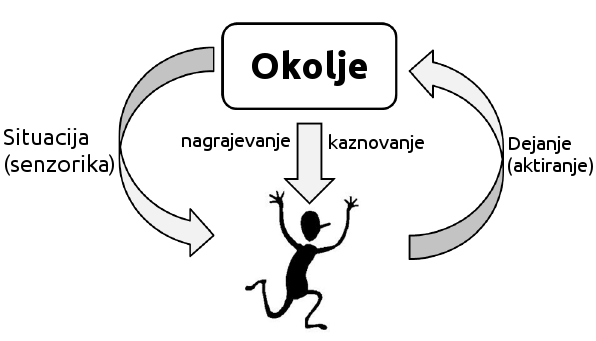
\includegraphics[scale=0.5]{slike/RLloop.png}
    \end{figure}
\end{frame}


\begin{frame}
    \frametitle{Kje je to uporabno?}
    \begin{itemize}
        \item Naučiti robota hoje
        \item Upravljati s portfeljem
        \item Igrati namizne igre
        \item Igrati katerekoli igre
        \item ...
    \end{itemize}
    Torej res praktično karkoli, kjer lahko cilj modeliramo kot numerične
    nagrade, ne poznamo pa optimalnih akcij za dostop do teh nagrad.
\end{frame}


\begin{frame}
    \frametitle{Problem}
    \begin{definicija}[Hipoteza o nagradi]
        Vse cilje je mogoče opisati kot maksimizacijo neke kumulativne numerične 
        nagrade.
    \end{definicija}

    \medskip

    \begin{itemize}
        \item To ni nujno res
    \end{itemize}
\end{frame}


\begin{frame}
    \frametitle{Primer: Križci in krožci 1}
    \begin{itemize}
        \item tu slika tistega loopa %(https://sl.wikipedia.org/wiki/Spodbujevano_učenje)
        \item \textbf{Stanje:} Kje je prazno, kje ">X"< in kje ">O"<
        \item \textbf{Agent:} Program, ki se odloča, kako igrati
        \item \textbf{Okolje:} Agentu sporoča nagrade in stanje
        \item \textbf{Nagrada:} Pozitivna za zmago, negativna za poraz
    \end{itemize}
\end{frame}


\begin{frame}
    \frametitle{Primer: Križci in krožci 2}
    \begin{itemize}
        \item Agent igra igre, posodablja svoje vrednosti stanj glede na odgovor okolja
        \item Kako naj to stori?
    \end{itemize}
\end{frame}


\begin{frame}
    \frametitle{Primer: Križci in krožci 3}
    \begin{itemize}
        \item Enostavna ideja:                                  
        \pause
        %
        $$
        V(s) \leftarrow V(s) + \alpha [R(s') + \gamma V(s') - V(s)]
        $$
        %                                       
        \pause
        \item $s$ je trenutno stanje                     
        \pause
        \item $V$ je vrednostna funkcija                 
        \pause
        \item $\alpha$ je velikost koraka (hitrost učenja) 
        \pause
        \item $R$ je nagrada   
        \pause
        \item $\gamma$ je diskontni faktor (pomemben je čas)    
        \pause
        \item $s'$ je stanje, ki sledi \textit{s}        
    \end{itemize}
\end{frame}


\begin{frame}
    \frametitle{Bistvo}
    %
    $$
    \text{nova ocena} \leftarrow \text{stara ocena} + \text{korak} 
    [\text{cilj/tarča} - \text{stara ocena}]
    $$
    %
    \medskip
    \begin{itemize}
        \item Tako ocenimo dano strategijo
        \item Kako pa strategijo dejansko spremenimo?
    \end{itemize}
\end{frame}


\begin{frame}
    \frametitle{Formalizacija: Markovski proces odločanja 1}
    \begin{definicija}[Markovska veriga]
        Skučajni proces $(S_t)_{t=0}^T$ na končnem verjetnostnem prostoru 
        $(\Omega, P)$ je \textbf{Markovska veriga}, če velja Markovska lastnost
        $$
        P(S_{t+1} = s_{t+1} | S_{t} = s_{t}, ..., S_0 = s_0) = P(S_{t+1} = s_{t+1} | S_{t} = s_{t})
        $$
    \end{definicija}
    \pause
    \medskip
    \begin{itemize}
        \item Prihodnost je neodvisna od preteklosti, če poznamo sedanjost
        \pause
        \item Definiramo $p_{ss'} := P(S_{t+1} = s' | S_{t} = s)$ in to združimo v matriko
                $\mathcal{P} := [p_{ss'}]_{s,s'\in \mathcal{S} }$, kjer je $\mathcal{S}$ 
                množica stanj
    \end{itemize}
    
\end{frame}


\begin{frame}
    \frametitle{Formalizacija: Markovski proces odločanja 2}
    %\begin{definicija}[Markovski proces]
    %    \textbf{Markovski proces} je par $(\mathcal{S}, \mathcal{P})$, kjer je
    %    \begin{itemize}
    %        \item $\mathcal{S}$ je (končna) množica stanj
    %        \item $\mathcal{P}$ je prehodna matrika
    %    \end{itemize}
    %\end{definicija}
    %\pause
    \begin{definicija}[Markovski proces odločanja]
        \textbf{Markovski proces odločanja} je nabor 
        $(\mathcal{S}, \mathcal{A}, \mathcal{P}, \mathcal{R}, \gamma)$, kjer je
        \begin{itemize}
            \item $\mathcal{S}$ je (končna) množica stanj
            \item $\mathcal{A}$ je (končna) množiza akcij oz. dejanj
            \item $\mathcal{P}$ je prehodna matrika, kjer $p_{ss'}^a = P(S_{t+1} = s' | S_{t} = s, A_t = a)$
            \item $\mathcal{R}$ je nagradna funkcija $\mathcal{R}_s^a = E[R_{t+1} | S_{t} = s, A_t = a]$
            \item $\gamma \in [0, 1]$ je diskontni faktor
        \end{itemize}
    \end{definicija}
\end{frame}


\begin{frame}
    \frametitle{Kako lahko to posplošimo}
    \begin{itemize}
        \item Koliko stanj imamo?
        \item Do kje lahko pridemo?
        \item Kdaj odpove?
        \item Kaj je rešitev?
    \end{itemize}
\end{frame}


%\begin{frame}
%    \bibliography{kratka}{}
%    \bibliographystyle{plain}
%\end{frame}


\begin{frame}
    \frametitle{Demonstracija: Križci in krožci}
    Morda kakšna slika/grafikon
\end{frame}


\begin{frame}
    \tikzstyle{block} = [rectangle, draw, 
    text width=5em, text centered, rounded corners, minimum height=4em]
\tikzstyle{line} = [draw, -latex]
\begin{tikzpicture}[node distance = 6em, auto, thick]
    \node [block] (Agent) {Agent};
    \node [block, below of=Agent] (Okolje) {Okolje};
        \path [line] (Agent.0) --++ (4em,0em) |- node [near start]{Akcija $a_t$} (Okolje.0);
        \path [line] (Okolje.190) --++ (-5em,0em) |- node [near start] {Novo stanje  $s_{t+1}$} (Agent.170);
        \path [line] (Okolje.170) --++ (-4.25em,0em) |- node [near start, right] {Nagrada $r_{t+1}$} (Agent.190);
\end{tikzpicture}
\end{frame}


\begin{frame}
    \frametitle{Ideje}
    \begin{itemize}
        \item Formalizacija, V, Q, pi, ...
    \end{itemize}
\end{frame}

% TODO: mentor 
% TODO: nagrade


\end{document}
